\documentclass[11pt,letterpaper]{article}
\usepackage[margin=1in]{geometry}
\usepackage[T1]{fontenc}
\usepackage{lmodern}
\usepackage{textcomp}
\usepackage{microtype}
\usepackage{booktabs}
\usepackage{tabularx}
\usepackage{graphicx}
\usepackage{float}
\usepackage{enumitem}
\usepackage[font=small,labelfont=bf]{caption}
\usepackage{pgfplots}
\pgfplotsset{compat=1.18}
\usepackage{fancyhdr}
\usepackage{xcolor}
\usepackage[hidelinks,
  pdftitle={TRACE-V: a PicoRV32 RISC-V core on SKY130, built by agentic AI and verified with independent open-source tools},
  pdfauthor={Raisul Islam}]{hyperref}

\definecolor{accent}{HTML}{2A78D6}
\definecolor{quiet}{HTML}{C3C2B7}

\setlength{\parindent}{0pt}
\setlength{\parskip}{0.6em}
\setlist{itemsep=0.2em,topsep=0.2em}
\setlength{\emergencystretch}{2em}
\pagestyle{fancy}
\fancyhf{}
\fancyhead[L]{TRACE-V v2.0}
\fancyfoot[C]{\thepage}
\renewcommand{\headrulewidth}{0.4pt}

\captionsetup{labelformat=empty}

\newcommand{\sk}[1]{\texttt{#1}}
\renewcommand{\_}{\textunderscore\penalty0\hskip0pt\relax}

\begin{document}

\begin{center}
{\LARGE\bfseries TRACE-V: a PicoRV32 RISC-V core on SKY130, built by agentic AI and verified with independent open-source tools\par}
\vspace{0.8em}
{Raisul Islam \textperiodcentered{} October 2026 \textperiodcentered{} Release v2.0\par}
\end{center}

\textit{TRACE-V: Traceable RISC-V --- AI-built, Checked, Evidenced.} The release is published at \url{https://github.com/raisul1212/trace-v} for non-commercial academic instruction and research.

Release v2.0 contains two implementations of the same design. The same RTL and the same constraint file were implemented by a commercial flow (Cadence Genus and Innovus) and by an open flow (Yosys and OpenROAD in LibreLane), and both builds are verified with the same open-source scripts. The commercial build is release v1.0.1, unchanged. Release v1.0.1 replaced the 8 ns route of v1.0 with an 8.25 ns route, which has a wider setup margin at the slow corner; the 8 ns release remains available at tag v1.0.

\section*{Abstract}
\begin{itemize}
\item \textbf{Commercial build (v1.0.1).} The PicoRV32 RV32I core was taken from RTL to block-level signoff on SkyWater sky130A at 8.25 ns (about 121 MHz). The requirements were set and the decisions were approved by the designer; implementation, verification, debugging and fixes were carried out by agentic AI on a commercial implementation flow. The routed block has 8,273 cells in a 357.42 $\times$ 355.64 \textmu m die.
\item Setup slack is +0.180 / +2.388 / +2.957 ns and hold slack is +0.716 / +0.214 / +0.034 ns at ss / tt / ff, after 0.25 ns clock uncertainty. Slew, capacitance and fanout violations are 0 at all three corners.
\item DRC (Magic and KLayout), antenna and LVS are clean, and both LEC steps are equivalent. The post-layout gate-level run of the golden program passes at 8.25 ns and the 4.125 ns control fails; a re-run in Xcelium with flop timing checks enforced also passes at 8.25 ns with 0 violations.
\item Static IR drop is 11 mV on VPWR and 11.6 mV on VGND against an 80 mV budget, and power is 13.0 mW (static, vectorless).
\item Six defects that each passed a tool's own report were found and corrected by agentic AI (section~\ref{sec:caught}). Signoff is at nominal RC (section~\ref{sec:rc}).
\item \textbf{Open build (v2.0).} The same RTL, under the byte-identical constraint file, was implemented with Yosys and OpenROAD in LibreLane 3.0.14, with private modifications to OpenROAD that are not published (section~\ref{sec:openimpl}). The die is 480.21 $\times$ 490.93 \textmu m at 45\% configured core utilization, with 144,143 transistors in logic cells.
\item In the shipped OpenSTA run, setup slack is +0.129 / +2.028 / +2.706 ns and hold slack is +0.744 / +0.235 / +0.054 ns at ss / tt / ff, with 0 slew, capacitance and fanout violations. DRC (Magic and KLayout), antenna and LVS are clean. Simulation passes at 8.25 ns in Icarus Verilog and in Xcelium with 0 timing violations, and both controls fail. Both equivalence steps are equivalent in Conformal. Static IR from OpenROAD PSM is 5.554 mV on VPWR and 5.573 mV on VGND (section~\ref{sec:openverify}).
\item Five defects found during the v2.0 work were fixed by agentic AI, among them a disagreement between two antenna checkers and a constraint mismatch (section~\ref{sec:v2defects}).
\item For each build, the release covers the following checks. Timing was signed off at three corners with 0.25 ns clock uncertainty. DRC was run with two independent decks, LVS was run against the routed netlist, and logic equivalence was checked at both synthesis and routing. Post-layout gate-level simulation was run with flop timing checks, and static IR was analyzed. Each verify script was checked to fail on a deliberately damaged input. Every reported figure is traceable to frozen, checksummed evidence. The physical, timing and simulation checks can be reproduced from either public package with open-source tools.
\end{itemize}

\section*{Background: PicoRV32}
PicoRV32 is a CPU core by Claire Xenia Wolf that implements the RISC-V RV32IMC instruction set. It can be configured as RV32E, RV32I, RV32IC, RV32IM or RV32IMC [1]. It is size-optimized, at 750--2,000 LUTs and 250--450 MHz on Xilinx 7-series FPGAs, and is intended mainly as an auxiliary processor in FPGA and ASIC designs [1]. Its average CPI is about 4, depending on the instruction mix. It is released under the ISC license [1].

It is a general-purpose CPU. RV32I is RISC-V's base 32-bit integer instruction set: 40 distinct instructions covering integer arithmetic, logic, shifts, compares, loads, stores, branches, jumps and system [2]. M (multiply/divide) and C (compressed) are optional extensions [2].

This build uses PicoRV32's default parameters, unchanged [1]:
\begin{itemize}
\item RV32I with all 32 registers and the cycle and instruction counters;
\item no multiply/divide, no compressed instructions, no interrupts and no co-processor interface;
\item a non-barrel shifter;
\item traps on misaligned accesses and illegal instructions.
\end{itemize}

The memory interface works as follows: the core asserts \sk{mem\_valid} and holds it until the memory asserts \sk{mem\_ready}. An optional look-ahead interface (\sk{mem\_la\_*}) announces a transfer one cycle early [1].

The process is SkyWater SKY130, an open-source 130 nm PDK; this design uses the \sk{sky130\_fd\_sc\_hd} standard-cell library [3].

\section{The design and target}\label{sec:design}
Sections~\ref{sec:design} to \ref{sec:results} describe the commercial build of v1.0.1; the open build is described in sections~\ref{sec:openimpl} to \ref{sec:side}. The design is PicoRV32, an RV32I RISC-V CPU core by Claire Xenia Wolf, released under the ISC license. The process is SkyWater sky130A, an open PDK, with \sk{sky130\_fd\_sc\_hd} standard cells. The target is a single clock of 8.25 ns (about 121 MHz) with 0.25 ns of clock uncertainty applied at every corner, and a fanout limit of 10 that is enforced.

PicoRV32 here is a 32-bit RISC-V core (RV32I). The routed block holds 87,237 transistors in 8,273 standard cells. The count comes from the sky130 SPICE model of every placed cell; filler, well-tap and antenna-diode cells add none.

\begin{center}
\begin{tabular}{@{}lll@{}}
\toprule
Corner & Temperature & Supply\\
\midrule
ss & 100 \textdegree C & 1.60 V\\
tt & 25 \textdegree C & 1.80 V\\
ff & $-$40 \textdegree C & 1.95 V\\
\bottomrule
\end{tabular}
\end{center}

The final routed block of the commercial build has the following size and activity figures.

\begin{center}
\begin{tabularx}{\linewidth}{@{}>{\raggedright\arraybackslash}p{0.34\linewidth}>{\raggedright\arraybackslash}X@{}}
\toprule
Quantity & Value\\
\midrule
Die & 357.42 $\times$ 355.64 \textmu m\\
Cells & 8,273 in the routed block, of which 176 are clock-tree buffers (7,845 in the synthesis netlist)\\
Cell area & 75,681 \textmu m\textsuperscript{2} in the routed block (71,909 \textmu m\textsuperscript{2} in the synthesis netlist)\\
Clock-tree insertion delay & 0.86--0.96 ns at ss, average 0.92 ns (Innovus CTS report)\\
Power & 13.0 mW, static and vectorless, 20\% input activity at 8.25 ns\\
Fanout limit & 10, enforced\\
\bottomrule
\end{tabularx}
\end{center}

\section{Flow and signoff bar}
Implementation and timing signoff of the v1.0.1 build use a commercial flow. Cadence Genus does synthesis, Innovus does place and route, Tempus produces timing and the SDF, Conformal checks logic equivalence, and Voltus computes IR drop.

Physical signoff uses open checkers, so that anyone can re-verify the layout without the commercial tools: Magic DRC, KLayout DRC with the sky130A\_mr deck, Magic antenna check, LVS with Magic and Netgen, and gate-level simulation in Icarus Verilog using the post-layout SDF. Icarus Verilog applies SDF path delays but not flop timing checks, so the same simulation is repeated in Cadence Xcelium with those checks enforced (section 3).

The signoff bar was set once by the designer, and the work was carried out against it by agentic AI without renegotiation per run:
\begin{itemize}
\item 0.25 ns clock uncertainty at ss, tt and ff, included in both setup and hold.
\item DRC clean in two independent decks.
\item Max transition, max capacitance and max fanout violations at 0.
\item Gate-level simulation and both LEC steps pass.
\item Static IR drop within budget, 80 mV on each rail (5\% of 1.6 V).
\end{itemize}

The open build of v2.0 was checked against the same bar (sections~\ref{sec:openimpl} and \ref{sec:openverify}).

The workload for simulation is a hand-assembled RV32I golden program of 9 instructions that sums 1 to 10 and stores 55.

\section{Results: commercial build}\label{sec:results}
Every check below passes at 8.25 ns for the commercial build. Setup and hold both include the 0.25 ns clock uncertainty.

\begin{center}
\small
\begin{tabularx}{\linewidth}{@{}>{\raggedright\arraybackslash}p{0.44\linewidth}>{\raggedright\arraybackslash}X@{}}
\toprule
Check & Result\\
\midrule
DRC, Magic & 0 violations\\
DRC, KLayout & 0 findings\\
Process antenna, Magic & 0 violations\\
LVS, Magic + Netgen, against the routed netlist & Matched; 8,492 / 8,492 nets\\
LEC, RTL $\to$ synthesized netlist (Conformal) & Equivalent; 1,916 compare points, 0 non-equivalent, aborted or unknown\\
LEC, synthesized $\to$ routed netlist (Conformal) & Equivalent; 1,864 compare points, 0 non-equivalent, aborted or unknown\\
Setup slack, ss / tt / ff & +0.180 / +2.388 / +2.957 ns; 0 violating endpoints\\
Hold slack, ss / tt / ff & +0.716 / +0.214 / +0.034 ns; 0 of 1,626 endpoints violating, input ports included\\
Max transition / capacitance / fanout & 0 / 0 / 0 at all three corners\\
Golden program on RTL & Pass\\
Golden program, post-layout gate level, ss SDF, 8.25 ns & Pass; the 4.125 ns control fails\\
Gate-level simulation with timing checks (Xcelium), 8.25 ns & Pass, 0 violations; the 4 ns control fails (76 violations)\\
Post-layout timing wall & Passes at 8 ns, fails at 6 ns\\
Static IR drop, VPWR / VGND & 11 mV / 11.6 mV; budget 80 mV each (5\% of 1.6 V)\\
\bottomrule
\end{tabularx}
\end{center}

\begin{figure}[H]
\centering
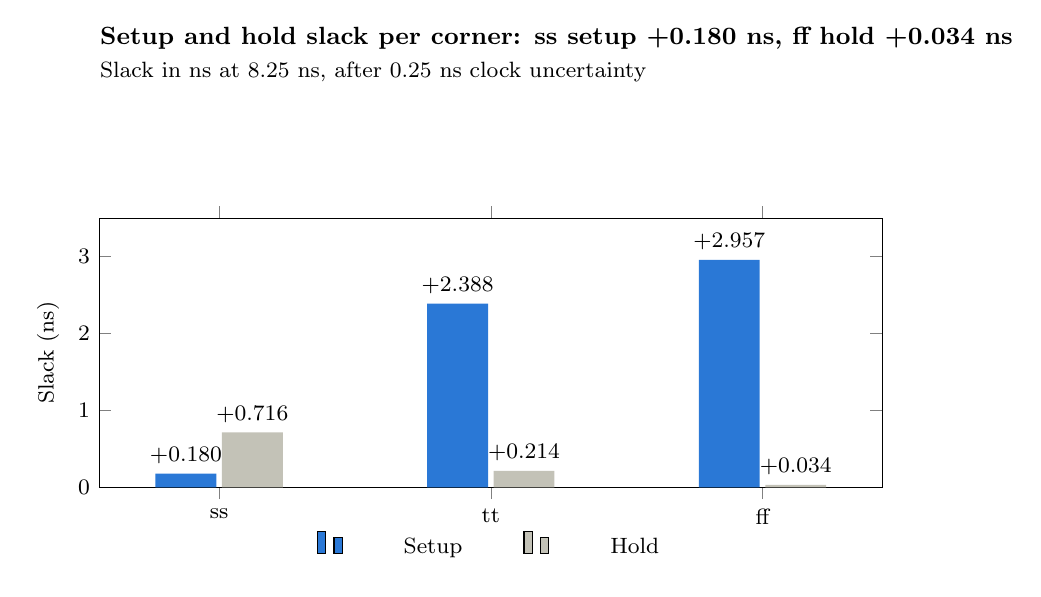
\begin{tikzpicture}
\node[anchor=south west,inner sep=0] at (0,5.55) {\small\bfseries Setup and hold slack per corner: ss setup +0.180 ns, ff hold +0.034 ns};
\node[anchor=south west,inner sep=0] at (0,5.15) {\footnotesize Slack in ns at 8.25 ns, after 0.25 ns clock uncertainty};
\begin{axis}[
  at={(0,0)}, anchor=south west,
  ybar, bar width=22pt, width=0.95\linewidth, height=5cm,
  symbolic x coords={ss,tt,ff}, xtick=data,
  ymin=0, ymax=3.5, ytick={0,1,2,3}, ylabel={Slack (ns)},
  enlarge x limits=0.22,
  nodes near coords,
  nodes near coords align={vertical},
  every node near coord/.append style={font=\footnotesize,/pgf/number format/.cd,fixed,precision=3,fixed zerofill,showpos},
  legend style={at={(0.5,-0.14)},anchor=north,legend columns=2,column sep=2em,draw=none,font=\footnotesize,/tikz/every legend image/.append style={xscale=0.6}},
  tick label style={font=\footnotesize}, label style={font=\footnotesize}]
\addplot[fill=accent,draw=none] coordinates {(ss,0.180) (tt,2.388) (ff,2.957)};
\addplot[fill=quiet,draw=none] coordinates {(ss,0.716) (tt,0.214) (ff,0.034)};
\legend{Setup,Hold}
\end{axis}
\end{tikzpicture}
\caption*{Setup and hold slack per corner at 8.25 ns, including 0.25 ns clock uncertainty; values from the signoff results table}
\end{figure}

Each simulation result has a control: the golden program passes at 8.25 ns and the 4.125 ns control fails, and the post-layout timing wall passes at 8 ns and fails at 6 ns.

Post-layout gate-level simulation was re-run in Cadence Xcelium with flop timing checks enforced, using the same netlist, SDF and testbench. Every timing check in the SDF was applied: 3,114 setup/hold checks and 3,114 pulse-width checks (100\%). At 8.25 ns the program passes with 0 timing-check violations, and at 10 ns it passes with 0. At 4 ns, the control, it times out with 76 violations.

\begin{figure}[H]
\centering
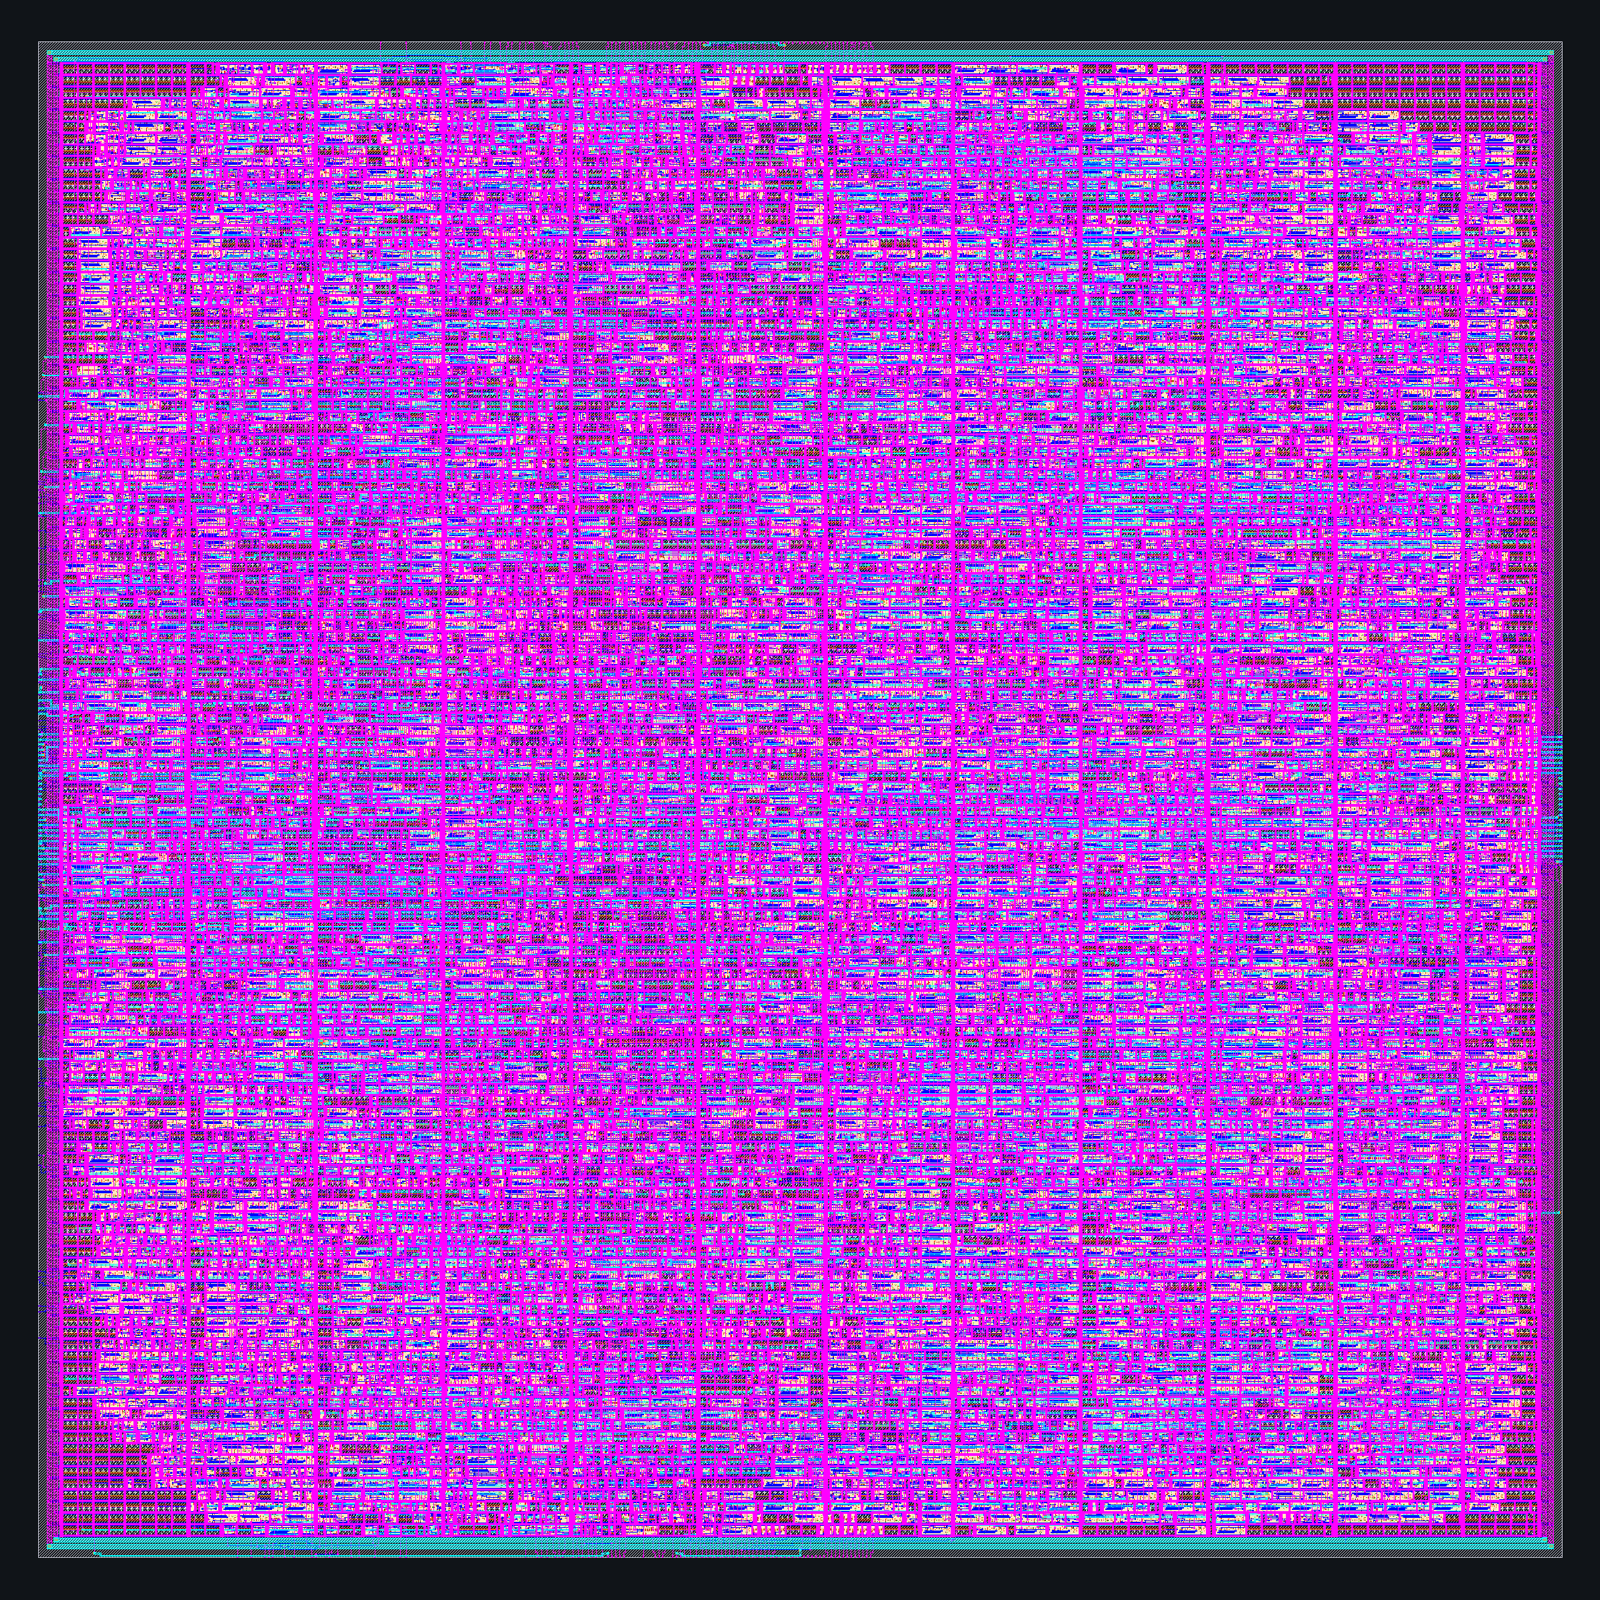
\includegraphics[width=0.78\linewidth]{figs/layout_825_1600.png}
\caption*{Figure 1. Commercial build: routed PicoRV32, 357.4 $\times$ 355.6 \textmu m, sky130A (KLayout render of the final GDS).}
\end{figure}

\section{Open-flow implementation}\label{sec:openimpl}
Release v2.0 adds a second implementation of the same RTL under the same constraint file. The file \sk{constraints/picorv32.sdc} is byte-identical in both packages (sha256 prefix \sk{14469a66864f3bda}). It sets an 8.25 ns clock with 0.25 ns uncertainty, a maximum fanout of 10 and a half-period I/O delay of 4.125 ns, because the testbench drives on the falling edge. The ports \sk{mem\_la\_*}, \sk{pcpi\_*}, \sk{eoi} and \sk{trace\_*} are unconstrained.

The open build was produced with LibreLane 3.0.14 in its Classic flow:
\begin{itemize}
\item Yosys synthesis, with \sk{SYNTH\_ABC\_BUFFERING} on and the \sk{DELAY 0} strategy;
\item OpenROAD placement and routing;
\item configured core utilization of 45\%, a clock-tree buffer spacing of 100 \textmu m, a maximum fanout of 10 and an antenna repair margin of 20;
\item a utilization sweep: at 55\% global routing fails with congestion and at 65\% timing repair fails, and at 40 to 45\% without the clock-tree buffer spacing the root clock buffer drives 16 loads against the limit of 10;
\item two antenna diodes inserted after routing with LibreLane's stock \sk{Odb.InsertECODiodes} step (section~\ref{sec:v2defects}).
\end{itemize}

\subsection*{Equivalent tools}
\begin{center}
\small
\begin{tabularx}{\linewidth}{@{}>{\raggedright\arraybackslash}p{0.27\linewidth}>{\raggedright\arraybackslash}X>{\raggedright\arraybackslash}X@{}}
\toprule
Step & Commercial build (v1.0.1) & Open build (v2.0)\\
\midrule
Logic synthesis & Cadence Genus 25.11 & Yosys 0.62 with ABC, inside LibreLane 3.0.14\\
Floorplan, placement, clock tree, routing, timing repair & Cadence Innovus 25.11 & OpenROAD (upstream \sk{dcf36133}) with private modifications, driven by LibreLane 3.0.14\\
Parasitic extraction for timing & Innovus, with the typical extraction file of the Cadence sky130 kit (nominal RC) & OpenRCX, inside OpenROAD\\
Signoff static timing & Cadence Tempus 23.10 & OpenSTA inside OpenROAD (upstream \sk{857316ff}), with private modifications\\
Static IR drop & Cadence Voltus & OpenROAD PSM with a private modification\\
Antenna repair & Innovus NanoRoute with an antenna margin & OpenROAD antenna repair, then two diodes added with LibreLane's stock \sk{Odb.InsertECODiodes} step\\
Logic equivalence & Cadence Conformal 24.10 & Cadence Conformal 24.10 (same tool)\\
Gate-level simulation with timing checks & Cadence Xcelium 24.03 & Cadence Xcelium 24.03 (same tool)\\
Release verification (\sk{verify/}) & Magic 8.3.623, KLayout 0.30.7, Netgen 1.5.316, OpenSTA 2.7.0, Icarus Verilog 13.0 & the same unmodified tools\\
\bottomrule
\end{tabularx}
\end{center}

\subsection*{Modifications inside the open-source tools}
Implementation used OpenROAD with private modifications that are not published. Every check an outsider runs uses unmodified open-source tools. The modifications are in four places.
\begin{enumerate}
\item \textbf{OpenROAD Resizer (\sk{rsz}): electrical repair and rebuffering.} After routing, repair uses the extracted parasitics, including zero-length shunt capacitances, in place of an estimate that had under-counted wire load by 2.2 to 2.4 times on two measured nets. Driver sizing uses the selected corner's model and the SDC slew limit, and fanout headroom accounts for antenna-diode loads.
\item \textbf{OpenSTA inside OpenROAD: parasitics and SDC.} The SPEF reader and the parasitic store give the Resizer the extracted RC network in a form its buffering model can use, and constraint checks ignore empty exception entries.
\item \textbf{OpenROAD PSM: static IR.} Voltage sources can be placed on a power pin's own routing layer as well as on the top layer. With this change, the PSM result on the commercial layout is within about 1 mV of Voltus.
\item \textbf{LibreLane: flow integration.} A post-route loop repairs electrical, setup and hold violations against freshly extracted parasitics, the flow exits with failure when a stated setup target is missed, and unchanged detailed wires are preserved.
\end{enumerate}
Yosys and ABC, Magic, KLayout, Netgen and Icarus Verilog were not modified. The antenna repair of the final layout uses a stock LibreLane step.

\begin{center}
\begin{tabularx}{\linewidth}{@{}>{\raggedright\arraybackslash}p{0.34\linewidth}>{\raggedright\arraybackslash}X@{}}
\toprule
Quantity & Value\\
\midrule
Die & 480.21 $\times$ 490.93 \textmu m\\
Standard-cell area & 122,928 \textmu m\textsuperscript{2}, of which 3,919 \textmu m\textsuperscript{2} are tap cells (119,009 \textmu m\textsuperscript{2} without them)\\
Cells & 10,801 logic cells, plus 3,132 taps, 494 antenna diodes, 19,498 decap and 11,766 fill\\
Transistors & 183,139, of which 144,143 are in logic cells and 38,996 in decap cells\\
LVS size & 11,237 devices and 10,944 nets\\
\bottomrule
\end{tabularx}
\end{center}

The transistor count uses the method of the shipped \sk{verify/transistors.sh}: the DEF components multiplied by the transistors per cell in the PDK cell SPICE. The commercial build has no decap cells, so its 87,237 transistors are all in logic cells. The open build was implemented with open\_pdks \sk{8afc8346}, the version LibreLane 3.0.14 selects, whose cell LEF and ss/tt timing libraries are byte-identical to those of open\_pdks \sk{97d08448}. Both builds were verified with \sk{97d08448}.

\section{Open-flow verification}\label{sec:openverify}
Every result in this section was measured on the final open layout. Timing, DRC, antenna, LVS and the Icarus Verilog simulation come from a run of the shipped open-source scripts; the other results name their tool.

\subsection*{Timing}
OpenSTA was run with the shipped \sk{verify/sta.tcl}, the nominal SPEF and the shared SDC. Slew, capacitance and fanout violations are 0 / 0 / 0 against library limits.

\begin{center}
\begin{tabular}{@{}lrr@{}}
\toprule
Corner & Setup slack & Hold slack\\
\midrule
ss & +0.129 ns & +0.744 ns\\
tt & +2.028 ns & +0.235 ns\\
ff & +2.706 ns & +0.054 ns\\
\bottomrule
\end{tabular}
\end{center}

The flow's own 9-corner signoff gives a max\_ss setup slack of +0.026 ns at max RC, a nom\_ss setup slack of +0.129 ns and a min\_ff hold slack of +0.051 ns. Slew, capacitance and fanout are 0 at all corners.

\subsection*{Physical checks}
\begin{itemize}
\item \textbf{DRC.} Magic reports 0 errors, and KLayout with the sky130A\_mr deck reports 0 findings.
\item \textbf{Antenna.} Magic \sk{antennacheck} reports 0 violations, with 30,900 gates analyzed.
\item \textbf{LVS.} Netgen, against a Magic extraction from the GDS, reports that the circuits match uniquely, with 11,237 devices and 10,944 nets.
\end{itemize}

\subsection*{Simulation}
Icarus Verilog with the post-layout SDF passes at 8.25 ns (RESULT 55, VERDICT PASS), and the 4.125 ns control fails (RESULT timeout).

Xcelium 24.03 was run with the SDF and flop timing checks (\sk{-neg\_tchk}), in the same harness as the v1.0.1 run. Of the setup/hold checks, 3,194 were annotated (100\%).
\begin{itemize}
\item At 8.25 ns the program passes (RESULT 55, VERDICT PASS) with 0 timing violations.
\item At 10 ns it passes with 0 violations.
\item At 4 ns, the control, it fails (RESULT timeout) with 2 timing violations.
\end{itemize}
For comparison, the commercial build has 0 violations at 8.25 ns with 3,114 checks, and its 4 ns control has 76 violations.

\subsection*{Equivalence}
Conformal LEC 24.10 was used for both steps.
\begin{itemize}
\item \textbf{RTL $\to$ Yosys netlist: equivalent.} There are 1,959 compare points, with 0 non-equivalent, 0 aborted and 0 unknown.
\item \textbf{Yosys netlist $\to$ routed netlist: equivalent.} There are 1,904 compare points, with 0 non-equivalent.
\end{itemize}
The RTL-to-netlist comparison required three steps:
\begin{enumerate}
\item flip-flop instances were renamed after their RTL registers, by a script that asserts identical cells and connections;
\item FSM encoding files were given for the two state registers that Yosys re-encoded: \sk{cpu\_state} from 8-bit one-hot to 7-bit one-hot, and \sk{mem\_wordsize} from 2-bit binary to 3-bit one-hot;
\item Conformal setup analysis merged 77 RTL registers (duplicates and registers the default configuration never uses) and treated 5 as constants.
\end{enumerate}
The control is the same comparison without the encoding files, in which 1,246 points are non-equivalent.

\subsection*{Static IR}
Static IR was computed with OpenROAD PSM, with private modifications, on the final layout. The conditions are ss, 100 \textdegree C and 1.6 V, with 20\% input activity, a power of 22.0 mW and 8 supply pins per net on met4/met5.
\begin{itemize}
\item The worst drop is 5.554 mV on VPWR and 5.573 mV on VGND. The average is 2.85 mV on VPWR and 2.75 mV on VGND.
\item The budget is 80 mV, 5\% of 1.6 V.
\item The controls behave as required. A single source gives 32.2 mV. Resistance multiplied by 3 gives 16.7 mV, and resistance multiplied by 25 gives 138.9 mV, which is over budget.
\item The method was validated on the commercial layout, where it gives 12.09 / 12.07 mV against Voltus 11.0 / 11.58 mV.
\end{itemize}
No Voltus run exists on the open layout.

\section{The two builds side by side}\label{sec:side}
\begin{center}
\small
\begin{tabularx}{\linewidth}{@{}>{\raggedright\arraybackslash}p{0.30\linewidth}>{\raggedright\arraybackslash}X>{\raggedright\arraybackslash}X@{}}
\toprule
 & Commercial (v1.0.1) & Open (v2.0)\\
\midrule
Clock / constraints & 8.25 ns, identical SDC & 8.25 ns, identical SDC\\
ss setup (shipped OpenSTA, nominal RC) & +0.280 ns (OpenSTA) / +0.180 ns (signoff timer) & +0.129 ns\\
ff hold & +0.034 ns & +0.054 ns\\
Die & 357.42 $\times$ 355.64 \textmu m & 480.21 $\times$ 490.93 \textmu m (45\% configured utilization)\\
Logic transistors & 87,237 & 144,143\\
DRC / antenna / LVS & 0 / 0 / match & 0 / 0 / match\\
Static IR (worst) & 11.0 / 11.58 mV (Voltus) & 5.55 / 5.57 mV (PSM)\\
Equivalence & RTL $\to$ netlist $\to$ routed (Conformal) & RTL $\to$ netlist $\to$ routed (Conformal)\\
\bottomrule
\end{tabularx}
\end{center}
The IR figures come from different tools. The PSM method, run on the commercial layout, gives 12.09 / 12.07 mV.

\subsection*{Step by step: tool and result in each flow}
\begin{center}
\small
\begin{tabularx}{\linewidth}{@{}>{\raggedright\arraybackslash}p{0.22\linewidth}>{\raggedright\arraybackslash}X>{\raggedright\arraybackslash}X@{}}
\toprule
Step & Commercial: tool, result & Open: tool, result\\
\midrule
Synthesis & Genus 25.11; 8,273 cells in the final layout (7,845 after synthesis) & Yosys 0.62 with ABC; 10,801 logic cells in the final layout\\
Place and route at 8.25 ns & Innovus 25.11; closes & OpenROAD, modified; closes (on the reference configuration with the default SDC, stock OpenROAD ends at $-$2.053 ns at max\_ss with 3,104 slew violations)\\
Timing, shipped OpenSTA script & ss setup +0.280 ns, ff hold +0.032 ns & ss setup +0.129 ns, ff hold +0.054 ns\\
Static IR, worst VPWR & Cadence Voltus; 11.0 mV & OpenROAD PSM, modified; 5.55 mV. On the commercial layout: 12.09 mV (unmodified PSM: 46.4 mV)\\
Logic equivalence (commercial tool in both) & Conformal 24.10; RTL $\to$ netlist $\to$ routed proven & Conformal 24.10; RTL $\to$ netlist $\to$ routed proven\\
Simulation with timing checks (commercial tool in both) & Xcelium 24.03; 0 violations, 3,114 checks & Xcelium 24.03; 0 violations, 3,194 checks\\
DRC / antenna / LVS (open tools in both) & Magic, KLayout, Netgen; 0 / 0 / match & Magic, KLayout, Netgen; 0 / 0 / match\\
\bottomrule
\end{tabularx}
\end{center}
Conformal and Xcelium were used for the open build as well. The open equivalence method did not prove the RTL-to-netlist step for this design (586 of 1,864 key points; the x-aware sequential proof was undecided after 2 h), and Icarus Verilog does not evaluate timing checks. The open build's implementation uses no commercial tool.

\section{Software developed for this work}\label{sec:software}
The design was implemented and verified by an agentic chip-design framework under the designer's direction. The software developed for it falls into three groups.
\begin{enumerate}
\item \textbf{Modifications inside open-source tools}, the four listed in section~\ref{sec:openimpl}. They are private and not published.
\item \textbf{Adapters of the agentic framework.} An adapter drives one tool step, reads its settings back, refuses a run it cannot verify, and records the result.
\begin{itemize}
\item Used for this release, commercial flow: adapters for Genus synthesis, Innovus place and route, Tempus timing, Voltus static IR and Conformal logic equivalence, behind an evidence registrar that writes each result to a ledger and freezes its inputs and outputs with checksums. The Xcelium simulation ran as a recorded job.
\item Used for this release, open flow: LibreLane runs with recorded configurations and hashes; the Conformal equivalence set-up (flip-flop renaming checked for identical structure, and FSM encoding files); PSM runs with a source-feed control and a weakened-grid control; and the stock-LibreLane ECO diode run.
\item Used for both builds: the verification scripts shipped in each folder's \sk{verify/}.
\item Developed alongside: an open logic-equivalence adapter over Yosys and ABC, whose run on this design is reported only as the negative result in the step-by-step table (586 of 1,864 key points; it did not prove the RTL-to-netlist step); and, not the source of any released number, an open static-IR adapter over OpenROAD PSM and a LibreLane runner and pre-flight plugin that read back every setting.
\end{itemize}
\item \textbf{Evidence handling.} Every cited result comes from a run whose inputs and outputs are frozen with checksums, and each verify script was checked to fail on a deliberately damaged input.
\end{enumerate}

\section{How the platform works}
The requirements were set and the decisions were approved by the designer. Implementation, verification, debugging and fixes were carried out by agentic AI against the signoff bar fixed in section 2. Five properties determine whether the results can be trusted.
\begin{enumerate}
\item \textbf{Every number traces to its source.} Every figure is traceable to the run and input files that produced it. Nothing is quoted from memory or from a log summary.
\item \textbf{Evidence is frozen.} Cited evidence is frozen and checksummed. The final signoff of the commercial build has 75 frozen evidence files (66 at signoff plus 9 from the Xcelium re-run), all verified, with 0 mismatches.
\item \textbf{Every physical, DRV and simulation check has a control.} A check is trusted after it has been shown to fail on a known-bad input. Gate-level simulation must fail at 4 ns. The antenna check must fail on a frozen known-bad layout. The slew, capacitance and fanout check must flag a deliberately overloaded net (a 5 pF load). The KLayout deck must fail on a planted violation. A check that passes every input is treated as broken.
\item \textbf{Refusal over silence.} A check that cannot run, or whose output cannot be read, is counted as a failure and never as a pass.
\item \textbf{Independent checkers.} The tool that builds something is always checked by at least one other tool, because a tool checking its own work shares its own blind spots. Innovus builds the layout, but DRC is run by Magic and by KLayout, and LVS by Magic and Netgen. LVS proves the layout matches the routed netlist; Conformal LEC then proves the routed netlist equals Genus' netlist, and Genus' netlist equals the RTL. The result is an unbroken chain of independent checks from the GDS back to the source code. In the open build, OpenROAD builds the layout, and the same open checkers and Conformal verify it.
\end{enumerate}

\section{What the platform caught}\label{sec:caught}
Each of the six defects below, found in the commercial flow, passed its tool's own report: the flow finished and the tool reported success. For each defect, the symptom, how it was found, the root cause and the fix are given. Three practices exposed the defects:
\begin{itemize}
\item \textbf{Read back.} Each result was read back from the design and compared with the requirement.
\item \textbf{Cross-checked.} Results that should agree were compared.
\item \textbf{Controlled.} Each check was shown to fail on a known-bad input before it was trusted.
\end{itemize}

\subsection{The fanout limit was declared and ignored}
\begin{itemize}
\item \textbf{Symptom.} The SDC set a maximum fanout of 10, yet Innovus finished with a 240-pin fanout violation. The tool's flow completed normally.
\item \textbf{How found.} It was flagged by the slew, capacitance and fanout check. That check is trusted because it flags a deliberately overloaded net (a 5 pF load).
\item \textbf{Root cause.} The router's optimizer and the clock-tree builder each need fanout repair enabled explicitly.
\item \textbf{Fix and numbers.} With repair enabled in both, the violation count is 0. The clock tree grew from 23 to 174 buffers, and insertion delay went from 0.46 to 0.95 ns (CTS report average).
\end{itemize}

\begin{figure}[H]
\centering
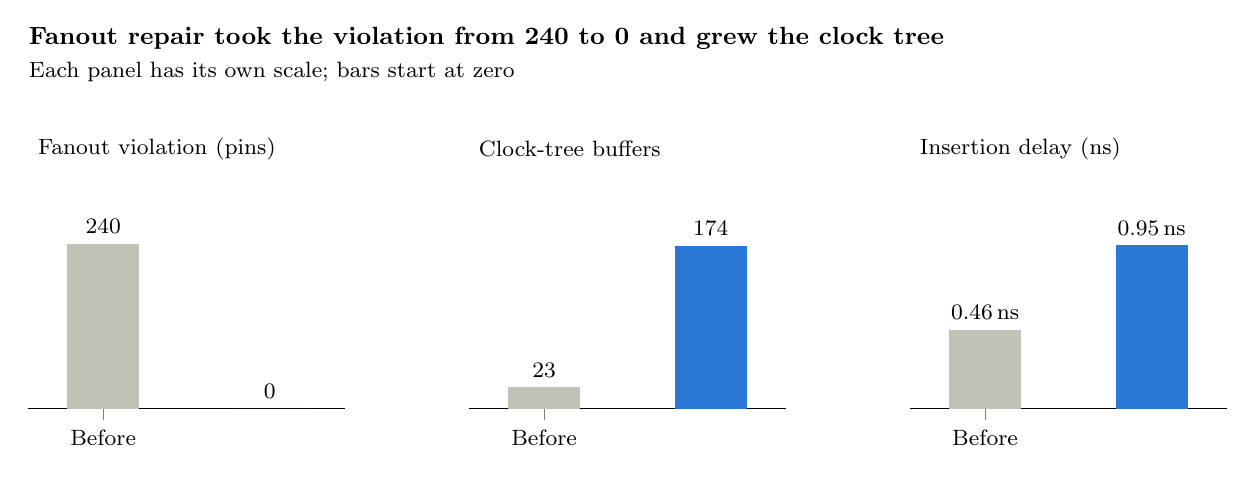
\begin{tikzpicture}
\node[anchor=south west,inner sep=0] at (0,4.55) {\small\bfseries Fanout repair took the violation from 240 to 0 and grew the clock tree};
\node[anchor=south west,inner sep=0] at (0,4.15) {\footnotesize Each panel has its own scale; bars start at zero};
\pgfplotsset{panel/.style={ybar, bar shift=0pt, bar width=26pt, width=5.6cm, height=4.2cm, symbolic x coords={Before,After}, xtick=data, ymin=0, enlarge x limits=0.45, nodes near coords, nodes near coords align={vertical}, every node near coord/.append style={font=\footnotesize}, tick label style={font=\footnotesize}, ytick=\empty, axis y line=none, axis x line*=bottom, title style={font=\footnotesize,align=left,anchor=west,at={(0,1.18)}}}}
\begin{axis}[panel, at={(0,0)}, anchor=south west, ymax=300, title={Fanout violation (pins)}, every node near coord/.append style={/pgf/number format/fixed,/pgf/number format/precision=0}]
\addplot[fill=quiet,draw=none] coordinates {(Before,240)};
\addplot[fill=accent,draw=none] coordinates {(After,0)};
\end{axis}
\begin{axis}[panel, at={(5.6cm,0)}, anchor=south west, ymax=220, title={Clock-tree buffers}, every node near coord/.append style={/pgf/number format/fixed,/pgf/number format/precision=0}]
\addplot[fill=quiet,draw=none] coordinates {(Before,23)};
\addplot[fill=accent,draw=none] coordinates {(After,174)};
\end{axis}
\begin{axis}[panel, at={(11.2cm,0)}, anchor=south west, ymax=1.2, title={Insertion delay (ns)}, nodes near coords={\pgfmathprintnumber[fixed,precision=2]{\pgfplotspointmeta}\,ns}]
\addplot[fill=quiet,draw=none] coordinates {(Before,0.46)};
\addplot[fill=accent,draw=none] coordinates {(After,0.95)};
\end{axis}
\end{tikzpicture}
\caption*{Fanout-repair fix, before and after; one panel per measure, each on its own scale}
\end{figure}

\subsection{STA passed while the gate-level simulation trapped}
\begin{itemize}
\item \textbf{Symptom.} After the fanout fix, setup was met at 8 ns, but the post-layout simulation hit a trap at 8 ns.
\item \textbf{How found.} The failing transaction that occurred earliest in the run was traced by agentic AI. The core misread an instruction it had been given correctly. The interface was then timed: the testbench drives memory on the falling edge, so \sk{mem\_ready} has half a cycle, and the path \sk{mem\_ready} $\to$ \sk{reg\_op1} was $-$1.87 ns.
\item \textbf{Root cause.} The constraints set no input or output delays, so STA gave those paths a full cycle. The larger clock tree had made them longer.
\item \textbf{Fix and numbers.} The SDC now states the environment the testbench models, with half-period input and output delays. The simulation then passes at 8 ns, and the input-port hold violations, worst $-$0.92 ns before, are gone.
\end{itemize}

\subsection{The gate-level simulation was all-X}
\begin{itemize}
\item \textbf{Symptom.} Every simulation failed, at every clock.
\item \textbf{How found.} A zero-delay positive control: the same netlist with no delays must pass, and it did not.
\item \textbf{Root cause.} The power-aware cell models had unconnected supplies, so every output resolved to X.
\item \textbf{Fix.} The simulated netlist now ties every cell's supply and body pins (VPWR, VGND, VPB, VNB) to constant 1 or 0 before simulation. A zero-delay run of the same netlist must pass; that positive control would have caught the all-X result.
\end{itemize}

\subsection{The antenna check could not fail}
\begin{itemize}
\item \textbf{Symptom.} The initial negative control for the antenna check passed. It contained a diode that was not needed, so it was not a violation, and the check had not been shown able to fail.
\item \textbf{Root cause.} The control was not a known-bad input.
\item \textbf{Fix.} It was replaced with a frozen known-bad layout that must fail. The final design has 0 antenna violations.
\end{itemize}

\subsection{A cell excluded from synthesis was re-inserted by place and route}
\begin{itemize}
\item \textbf{Symptom.} KLayout reported one npc.2 violation (0.16 \textmu m against 0.27 \textmu m) on the initial 8.25 ns route, while Magic DRC was clean.
\item \textbf{How found.} The violation was reported by the second, independent DRC deck.
\item \textbf{Root cause.} The cell \sk{sky130\_fd\_sc\_hd\_\_and2\_0} has an NPC edge 0.16 \textmu m inside its boundary. It was excluded in Genus, but restructuring in Innovus re-inserted it.
\item \textbf{Fix.} The exclusion is applied in Innovus as well, and a post-route count of excluded cells must be zero.
\end{itemize}

\subsection{An antenna violation remained after the router's repair}
\begin{itemize}
\item \textbf{Symptom.} One net had an antenna ratio of 403.85 against a limit of 400.
\item \textbf{How found.} The violation was reported by the open antenna check.
\item \textbf{Root cause.} The router's repair did not bring the net below the limit.
\item \textbf{Fix.} The router now repairs to 96\% of the limit.
\end{itemize}

\subsection*{Defects found and fixed during the v2.0 work}\label{sec:v2defects}
The same practices were applied to the open flow. Five defects were found and fixed by agentic AI.

\subsubsection*{Constraint mismatch}
\begin{itemize}
\item \textbf{Symptom.} The open flow initially used LibreLane's default SDC, with a 1.65 ns I/O delay.
\item \textbf{How found.} The build was timed under the commercial SDC, where it failed ss setup by $-$2.294 ns at the input \sk{resetn}.
\item \textbf{Fix.} The build was re-run under the identical SDC, and it closes.
\end{itemize}

\subsubsection*{Fragile closure}
\begin{itemize}
\item \textbf{Symptom.} Before the timing-repair modification, an 8.25 ns closure at +0.019 ns fell to $-$0.195 ns after a small placement change (wire-length weight 0.25 $\to$ 0.3).
\item \textbf{Fix.} After the modification, the same perturbation passes at +0.039 ns.
\end{itemize}

\subsubsection*{Antenna checker disagreement}
\begin{itemize}
\item \textbf{Symptom.} OpenROAD reported 0 antenna violations, and Magic flagged 3 gates on an earlier candidate layout and 2 on the release layout.
\item \textbf{Root cause.} Magic counts metal3 that reaches a gate through metal4 alone as connected at the metal3 step.
\item \textbf{Proof.} On net \sk{\_06165\_}, the computed ratio is 1,662.6 against Magic's reported 1,666.5. Erasing the metal4 bridge in a copy of the layout takes Magic to 0.
\item \textbf{Fix and numbers.} On the released 45\% layout, Magic flagged two gates, and two diodes were added with a stock ECO step. The diode count went from 492 to 494, the area grew by 5 \textmu m\textsuperscript{2}, and the max\_ss setup slack went from +0.027 to +0.026 ns.
\item \textbf{Alternative considered and not used.} A patched mode added 2,098 diodes (+9.7\% area).
\end{itemize}

\subsubsection*{Verification environment}
\begin{itemize}
\item \textbf{Symptom.} With a newer PDK than the pinned one, the diode cells failed LVS.
\item \textbf{Root cause.} LVS and antenna results depend on the PDK version.
\item \textbf{Fix.} The README pins open\_pdks \sk{97d08448}, and the scripts must be run with it.
\end{itemize}

\subsubsection*{Equivalence setup}
\begin{itemize}
\item \textbf{Symptom.} Re-encoded state machines and constant registers defeat a plain key-point comparison: 1,268 non-equivalent points, then 1,200, until they were handled.
\item \textbf{Fix.} The three steps in section~\ref{sec:openverify} (register renaming, FSM encoding files and Conformal setup analysis) resolve it.
\end{itemize}

\section{Power and IR: commercial build}
For the commercial build, static IR drop from Voltus is 11 mV on VPWR and 11.6 mV on VGND. The budget is 80 mV on each rail, 5\% of 1.6 V, so the block uses about 14\% of the budget on VPWR. The legend of the VPWR map spans 1.588 to 1.600 V, and the worst drop is 11 mV. Power is 13.0 mW, static and vectorless, assuming 20\% input activity at 8.25 ns.

\begin{figure}[H]
\centering
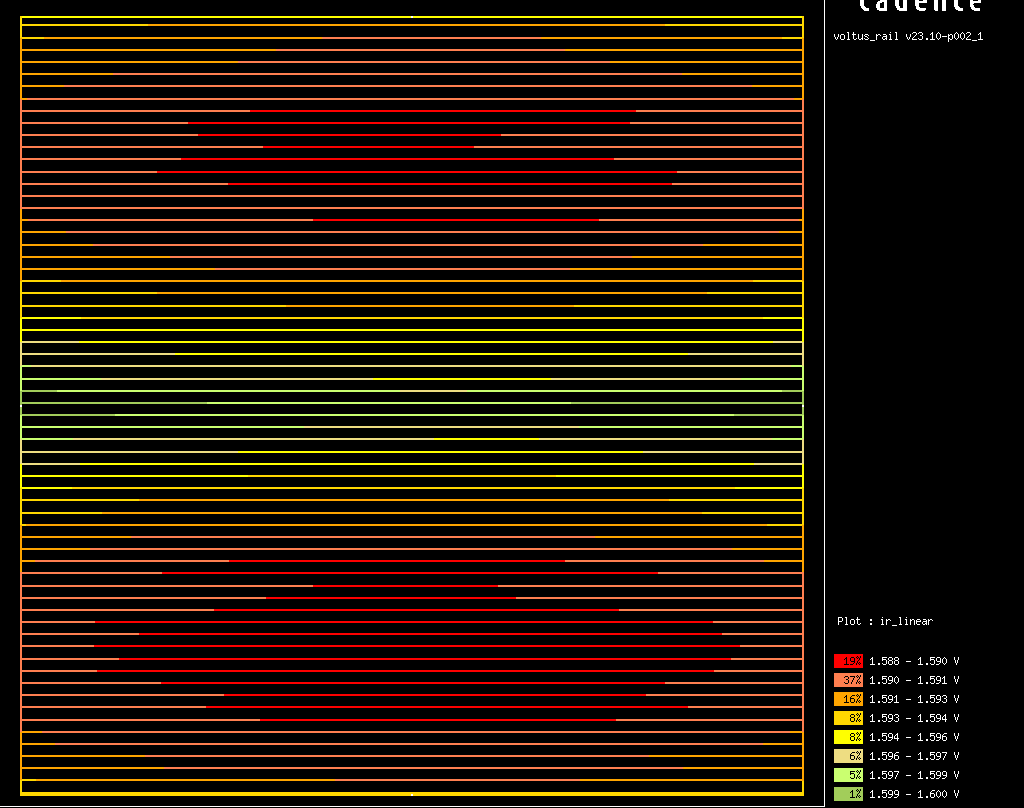
\includegraphics[width=0.78\linewidth]{figs/ir_vpwr_825.png}
\caption*{Figure 2. Commercial build: static IR map of VPWR (Voltus, vectorless): legend 1.588--1.600 V, worst drop 11 mV against an 80 mV budget.}
\end{figure}

\section{Independent RC cross-check: commercial build}\label{sec:rc}
Signoff extraction of the commercial build is at nominal RC, because the Cadence sky130 kit ships a typical extraction file and no other corner. To bound what that leaves out, the final layout was re-extracted with OpenRCX and timed with OpenSTA, tools independent of the signoff flow.

\begin{figure}[H]
\centering
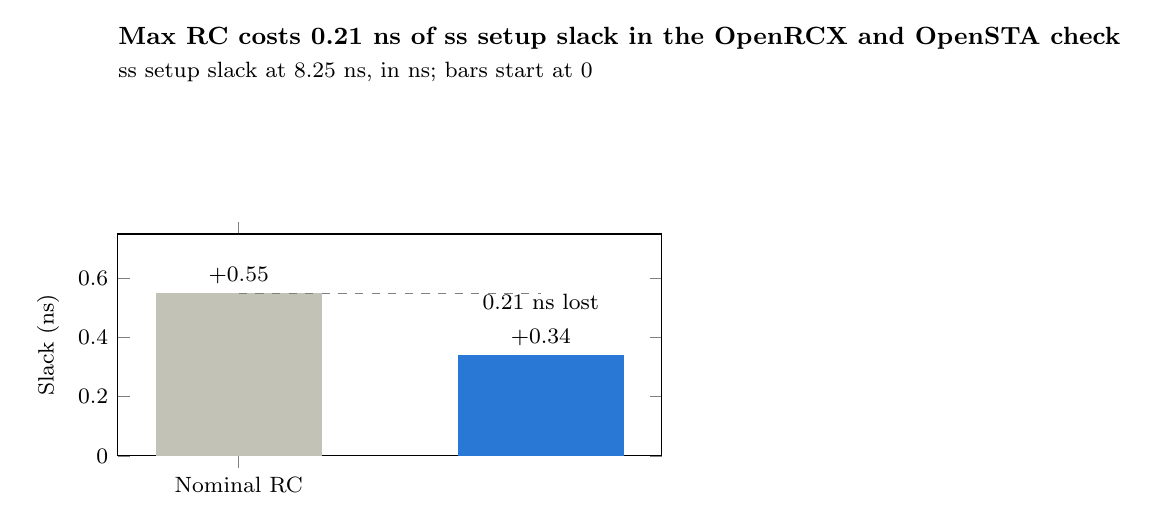
\begin{tikzpicture}
\node[anchor=south west,inner sep=0] at (0,5.15) {\small\bfseries Max RC costs 0.21 ns of ss setup slack in the OpenRCX and OpenSTA check};
\node[anchor=south west,inner sep=0] at (0,4.75) {\footnotesize ss setup slack at 8.25 ns, in ns; bars start at 0};
\begin{axis}[
  at={(0,0)}, anchor=south west,
  ybar, bar shift=0pt, bar width=60pt, width=0.7\linewidth, height=4.4cm,
  symbolic x coords={Nominal RC,Max RC}, xtick=data,
  ymin=0, ymax=0.75, ytick={0,0.2,0.4,0.6}, ylabel={Slack (ns)},
  enlarge x limits=0.4,
  nodes near coords, nodes near coords align={vertical},
  every node near coord/.append style={font=\footnotesize,/pgf/number format/.cd,fixed,precision=2,fixed zerofill,showpos},
  tick label style={font=\footnotesize}, label style={font=\footnotesize}]
\addplot[fill=quiet,draw=none] coordinates {(Nominal RC,0.55)};
\addplot[fill=accent,draw=none] coordinates {(Max RC,0.34)};
\draw[dashed,gray] (axis cs:Nominal RC,0.55) -- (axis cs:Max RC,0.55);
\node[font=\footnotesize,anchor=south] at (axis cs:Max RC,0.46) {0.21 ns lost};
\end{axis}
\end{tikzpicture}
\caption*{ss setup slack at 8.25 ns, nominal against max RC; OpenRCX re-extraction timed in OpenSTA}
\end{figure}

ss setup at 8.25 ns is +0.55 ns with nominal RC and +0.34 ns with max RC, so max RC costs 0.21 ns. The ff hold check with min RC is +0.03 ns and is met.

The figures of about $-$0.03 ns at max RC and about 8.3 ns to close are an estimate combining two extractors: the 0.21 ns shift measured with OpenRCX and OpenSTA is applied to the signoff margin of +0.180 ns.

\section{Cost}
The figures below describe the commercial flow of v1.0.1. All counts run from 1 Oct through the 8 ns signoff (7 Oct, 16:15 EDT), and the figures are held as frozen evidence. The 8.25 ns re-run added 21 cluster jobs and 2.0 h of wall time.

\begin{center}
\begin{tabularx}{\linewidth}{@{}>{\raggedright\arraybackslash}p{0.42\linewidth}>{\raggedright\arraybackslash}X@{}}
\toprule
Item & Figure\\
\midrule
Calendar time & 1 to 7 Oct 2026, from the start of the commercial flow on the open sky130 PDK to block signoff\\
One full signoff pass, synthesis through the clock sweep & 38 min of compute, 45 min end to end\\
Commercial cluster jobs & 62 jobs, 5.1 h total wall time\\
Agentic AI calls & 2,907\\
Output tokens & 1.26 M\\
Input tokens & 0.89 B cached tokens read, 32 M written to cache, about 6.5 k uncached\\
\bottomrule
\end{tabularx}
\end{center}

About 3.1 hours of designer interaction were spent over 7 days, in 86 messages. The requirements were set and each decision was approved by the designer. Implementation, verification, debugging and fixes were carried out by agentic AI. Times were measured from message timestamps, with gaps under 20 minutes counted as work. Token and time figures are upper bounds, because parallel work outside this design was included.

\section{Limitations}
Packaging, electromigration, metal fill, pad frame, foundry precheck and dynamic IR were outside the scope of this block-level release. Items 1 and 3 apply to the commercial build; items 2 and 4 apply to both builds; items 5 and 6 apply to the open build.
\begin{enumerate}
\item \textbf{Nominal RC.} Signoff is at nominal RC (section~\ref{sec:rc}).
\item \textbf{I/O timing.} I/O timing is set to the testbench's half-cycle memory protocol. The look-ahead outputs (\sk{mem\_la\_*}) and the other outputs that the testbench does not sample are unconstrained.
\item \textbf{Thin margins.} The margins are ss setup +0.180 ns and ff hold +0.034 ns, after 0.25 ns uncertainty.
\item \textbf{Workload.} The post-layout simulation runs one 9-instruction program covering 6 of 40 RV32I opcodes; LEC and STA cover the whole design.
\item \textbf{Open-build IR.} The static IR of the open build comes from OpenROAD PSM with private modifications. No Voltus run exists on the open layout; the PSM method was validated on the commercial layout.
\item \textbf{Commercial checks of the open build.} The equivalence results (Conformal) and the timing-checked simulation (Xcelium) of the open build use commercial tools and are not regenerated by the open scripts.
\end{enumerate}

\section{Reproducing}
The repository at \url{https://github.com/raisul1212/trace-v} contains two self-contained packages, \sk{commercial/} and \sk{open/}, each with its own verify/ scripts, reports and SHA256SUMS. Each package contains:
\begin{itemize}
\item rtl and netlists;
\item layout: the GDS, byte-identical to the one used at signoff, and the DEF;
\item constraints, SPEF and SDF;
\item the testbench;
\item verify/ scripts for the open-source tools;
\item the reports from the open-tool verification run;
\item SHA256SUMS.
\end{itemize}
The repository root holds the README, LICENSE, NOTICE, LICENSES/ and docs/ with the presentation and whitepaper PDFs.

The physical checks of each package can be re-run with the open-source tools and the scripts in its verify/, inside the LibreLane 3.0.14 container, with open\_pdks \sk{97d08448} installed by volare. LVS and antenna results depend on the PDK version, so the pinned PDK is required. The commercial-tool signoff figures (Genus, Innovus, Tempus, Conformal, Voltus and Xcelium) and the OpenROAD PSM IR figures are stated in this paper and are not regenerated by the open scripts.

\textbf{License.} The released design files are licensed for non-commercial academic instruction and research; commercial use needs written permission. \sk{picorv32.v} keeps its ISC license, and the SKY130 PDK data keep Apache-2.0. For research collaboration or licensing inquiries about the framework, contact Raisul Islam, raisul@purdue.edu.

\section*{References}
\raggedright
[1] C. X. Wolf, ``PicoRV32 --- A Size-Optimized RISC-V CPU,'' YosysHQ, \url{https://github.com/YosysHQ/picorv32} (README).

[2] A. Waterman and K. Asanovi\'c (eds.), ``The RISC-V Instruction Set Manual, Volume I: Unprivileged ISA,'' RISC-V International.

[3] SkyWater Technology and Google, ``SkyWater SKY130 PDK,'' \url{https://github.com/google/skywater-pdk}; open\_pdks 1.0.471, \url{https://github.com/RTimothyEdwards/open_pdks}.

\end{document}
